% Provenance (never printed): see sources/outline_sources.md (Year 1: grain size and sorting;
% bedforms and sedimentary structures; fluvial, deltaic, shoreline and deep-sea deposits).
% Exercise and problem values in the Book 3 scratch calculator calc/ch21.py; figure data
% from figdata/bachelor-1/grain_size.py. Meander and delta are Book 1's (g5), sediment and
% sedimentary layer Book 1's (g7), beach Book 1's (g9); the loads, settling, the threshold
% of motion and the Hjulstrom diagram are ch. 20's; the vector mean is ch. 6's. Facies
% models and Walther's law belong to the Year 3 volume (prose pointer only). Pelagic
% sediments are ch. 22's.
\chapter{Clastic Sediments and Their Environments}\label{ch:b1:clastic-sediments}

Pick up a handful of sand on a beach and let it run through your fingers: the
grains are all nearly the same size, rounded and clean, and they flow like
water. A few hundred kilometres inland, at the foot of a hill left by an old
glacier, the ground is a stiff mixture of boulders, pebbles, sand and mud,
without order. The two deposits are made of the same kind of debris, broken
from the same kinds of rock; what separates them is how the grains travelled and
where they came to rest. A wave that runs up and down a beach thousands of
times a day sorts the grains by size, carries the fine ones away and rounds the
rest; ice carries everything it picks up and drops it all together when it
melts. This chapter learns to read such stories from the grains themselves,
from the structures they build on the beds of rivers and seas, and from the
order in which the deposits are stacked.

\begin{recall}
A sediment is loose material laid down by water, wind or ice, and over time
sediments pile up in layers that harden into sedimentary rock (Book~1, grades~6
and~7). A river that swings from side to side across its floodplain forms
meanders; where it enters the sea or a lake and drops its load, it builds a
delta; waves pile sand into beaches and move it along the shore by longshore
drift (Book~1, grades~5 and~9). A river carries its load as \omterm{def:b1:erosion-transport:load}{bed load}, \omterm{def:b1:erosion-transport:load}{suspended
load} and \omterm{def:b1:erosion-transport:load}{dissolved load}; a grain sinks at its \omterm{def:b1:erosion-transport:settling}{settling velocity}; it starts to
move when the \omterm{def:b1:erosion-transport:bed-shear}{bed shear stress} passes its \omterm{def:b1:erosion-transport:threshold}{threshold of motion}, and the
\omterm{def:b1:erosion-transport:hjulstrom}{Hjulström diagram} shows the mean velocities of erosion, transport and deposition
against the grain size (\cref{ch:b1:erosion-transport}). The vector mean of a
set of directions is the direction of the sum of their unit vectors
(\cref{def:b1:field-lab-methods-1:mean-orientation}).
\end{recall}

\section{Grain size and sorting}\label{sec:b1:clastic-sediments:grain-size}

The size of the grains is the first thing a geologist records in a clastic
sediment, one made of fragments of older rocks, because it measures the energy
of the current that laid them down. Grain sizes in nature span more than seven
orders of magnitude, from boulders metres across to clay particles a thousandth
of a millimetre wide, and they are measured on a scale of ratios.

\begin{definition}[Grain-size scale, phi scale]\label{def:b1:clastic-sediments:grain-size}
The \emph{grain-size scale}\index{grain-size scale} of sedimentology divides the
diameters of grains into classes whose limits double from one class to the
next, starting from \qty{1}{mm}; each class is named (sand, silt\ldots). The
\emph{phi scale}\index{phi scale} expresses a diameter $d$ by
\[
  \varphi = -\log_2 \frac{d}{\qty{1}{mm}},
\]
so that $d = 2^{-\varphi}$~mm: \qty{1}{mm} is $\varphi = 0$, \qty{2}{mm} is
$\varphi = -1$, \qty{0.25}{mm} is $\varphi = 2$, and finer grains have larger
values of $\varphi$.
\end{definition}
% ledger: folk:udden-krumbein, folk:wentworth-classes, usgs:wentworth-phi

On the \omterm{def:b1:clastic-sediments:grain-size}{phi scale} every class of the \omterm{def:b1:clastic-sediments:grain-size}{grain-size scale} is one unit wide: a class
running from $d$ to $2d$ runs from $\varphi$ to $\varphi - 1$. The main classes,
with the names in common use, are listed in \cref{tab:b1:clastic-sediments:classes}.

\begin{table}[htbp]
\centering\small
\begin{tabular}{@{}lll@{}}
\hline
class & diameter (\si{mm}) & $\varphi$ \\
\hline
boulder & above 256 & below $-8$ \\
cobble & 64 to 256 & $-6$ to $-8$ \\
pebble & 4 to 64 & $-2$ to $-6$ \\
granule & 2 to 4 & $-1$ to $-2$ \\
sand (very coarse, coarse, medium, fine, very fine) & $1/16$ to 2 & 4 to $-1$ \\
silt (coarse, medium, fine, very fine) & $1/256$ to $1/16$ & 8 to 4 \\
clay & below $1/256$ (\qty{3.9}{\micro m}) & above 8 \\
\hline
\end{tabular}
\caption{The grain-size classes. The five classes of sand are each one phi
unit wide, from very coarse (1 to \qty{2}{mm}) to very fine ($1/16$ to
$1/8$~mm), and so are the four classes of silt. Some workers put the lower
limit of silt at 9 rather than $8\,\varphi$. Gravel is the general name for
grains coarser than \qty{2}{mm}, and mud for the mixture of silt and clay.}
\label{tab:b1:clastic-sediments:classes}
\end{table}
% ledger: folk:wentworth-classes, usgs:wentworth-phi

The word \emph{clay} has two meanings in this book: here it is a size class, in
\cref{ch:b1:weathering-clays} a family of \omterm{def:b1:rock-forming-minerals:mineral}{minerals}. Most clay-sized particles
are \omterm{def:b1:weathering-clays:clay-mineral}{clay minerals} and most \omterm{def:b1:weathering-clays:clay-mineral}{clay minerals} are clay-sized, but the two do not
coincide: quartz ground very fine is clay-sized, and a \omterm{def:b1:weathering-clays:clay-mineral}{kaolinite} book can be
the size of silt.

\emph{Measuring the sizes.} Gravel is measured grain by grain with calipers.
Sand is sieved: a stack of sieves with meshes at every whole or half phi unit
is shaken, and each sieve's catch is weighed. Silt and clay, finer than
$4\,\varphi$, are measured by settling: the sediment is stirred into water, and
since each grain sinks at a speed set by its size (Stokes' law,
\cref{prop:b1:erosion-transport:stokes}), the mass still in suspension at a
given depth and time tells how much of the sample is finer than a given
diameter. Laser instruments that measure the scattering of light by the grains
are now common too. The result is a list of the weight per cent in each class.

\begin{definition}[Mean grain size, sorting]\label{def:b1:clastic-sediments:sorting}
Let the grain sizes of a sediment, in phi units, have the distribution given by
the weight in each class. Its \emph{mean grain size}\index{mean grain size} is
the mean of that distribution, and its \emph{sorting}\index{sorting} is the
spread of the distribution, measured by its standard deviation in phi units: a
sediment is well sorted when its grains are nearly all of one size, and poorly
sorted when they cover many classes. Both are computed either from the
percentages in the classes, by the method of moments, or from the cumulative
curve, by the graphic measures of Folk:
\[
  M_z = \frac{\varphi_{16} + \varphi_{50} + \varphi_{84}}{3}, \qquad
  \sigma_I = \frac{\varphi_{84} - \varphi_{16}}{4} + \frac{\varphi_{95} - \varphi_{5}}{6.6},
\]
where $\varphi_p$ is the size in phi units than which $p$ per cent of the sample
is coarser.
\end{definition}
% ledger: folk:graphic-measures

\begin{method}[Mean and sorting from a sieve analysis]\label{met:b1:clastic-sediments:graphic}
\begin{enumerate}
  \item List the weight per cent $w_i$ in each class, from the coarsest to the
        finest, and check that the sum is \qty{100}{\percent} (or divide by it).
  \item \emph{Method of moments.} With $x_i$ the mid-point of class $i$ in phi
        units, compute the mean $m = \sum w_i x_i / 100$ and the standard
        deviation $s = \sqrt{\sum w_i (x_i - m)^2 / 100}$.
  \item \emph{Graphic measures.} Accumulate the percentages to get the weight
        per cent coarser than each class limit, and plot it against $\varphi$:
        this is the cumulative curve.
  \item Read on it, by linear interpolation between class limits, the sizes
        $\varphi_5$, $\varphi_{16}$, $\varphi_{50}$, $\varphi_{84}$ and
        $\varphi_{95}$.
  \item Compute $M_z$ and $\sigma_I$ (\cref{def:b1:clastic-sediments:sorting}),
        convert $M_z$ to millimetres by $d = 2^{-M_z}$, and name the \omterm{def:b1:clastic-sediments:sorting}{sorting}
        from the scale below.
\end{enumerate}
\end{method}

The two methods give nearly the same answers, and the reason is the following
property.

\begin{proposition}[Graphic measures of a normal distribution]\label{prop:b1:clastic-sediments:normal}
If the sizes of a sediment, in phi units, are distributed normally with mean
$\mu$ and standard deviation $\sigma$, then $M_z = \mu$ and $\sigma_I = 0.996\,\sigma$.
\end{proposition}

\begin{proof}
For a normal distribution, the fraction of values below $\mu + z\sigma$ depends
only on $z$; the fraction below $\mu + 0.9945\,\sigma$ is \qty{84}{\percent}
and below $\mu + 1.6449\,\sigma$ it is \qty{95}{\percent} (values of the normal
distribution, admitted). By symmetry, $\varphi_{50} = \mu$, $\varphi_{16} = \mu -
0.9945\,\sigma$, $\varphi_{84} = \mu + 0.9945\,\sigma$, $\varphi_5 = \mu -
1.6449\,\sigma$ and $\varphi_{95} = \mu + 1.6449\,\sigma$ (the percentiles count
the coarser part, that is the smaller $\varphi$, but the distribution is
symmetric). Then $M_z = (3\mu)/3 = \mu$ and
\[
  \sigma_I = \frac{2 \times 0.9945\,\sigma}{4} + \frac{2 \times 1.6449\,\sigma}{6.6}
  = (0.4972 + 0.4985)\,\sigma = 0.996\,\sigma. \qedhere
\]
\end{proof}

The constant 6.6 in Folk's formula is chosen for this: the interval from the
5th to the 95th percentile spans $3.29$ standard deviations of a normal
distribution, and the formula averages the estimates of $\sigma$ from the two
intervals, $(\varphi_{84}-\varphi_{16})/2$ and $(\varphi_{95}-\varphi_5)/3.3$.
Using the tails as well as the central two-thirds of the curve makes $\sigma_I$
sensitive to the coarse and fine admixtures that tell the most about how a
sediment was deposited.

\begin{omfigure}
\begin{tikzpicture}[font=\small]
% grain-size histograms and cumulative curves of two invented samples (figdata/bachelor-1/grain_size.py)
\begin{axis}[name=a, width=7.3cm, height=6cm, xmin=-5.5, xmax=10.5, ymin=0, ymax=90,
    xlabel={grain size $\varphi$}, ylabel={weight per cent in the class},
    title={\footnotesize (a) histograms}, xtick={-4,-2,...,10}, ytick={0,20,...,80},
    legend style={at={(0.03,0.97)}, anchor=north west, font=\scriptsize}, legend cell align=left]
  \addplot[ybar interval, fill=omDef!35, draw=omDef, area legend] table[x=phi, y=wt] {figdata/out/bachelor-1-grain_size-step-beach.dat} \closedcycle;
  \addplot[const plot, fill=omThm!20, draw=omThm, fill opacity=0.6, area legend] table[x=phi, y=wt] {figdata/out/bachelor-1-grain_size-step-till.dat} \closedcycle;
  \legend{beach sand (half-phi classes), till (whole-phi classes)}
\end{axis}
\begin{axis}[at={(a.east)}, anchor=west, xshift=1.6cm, width=7.3cm, height=6cm, xmin=-5.5, xmax=10.5, ymin=0, ymax=100,
    xlabel={grain size $\varphi$}, ylabel={weight per cent coarser},
    title={\footnotesize (b) cumulative curves}, xtick={-4,-2,...,10}, ytick={0,16,50,84,100},
    grid=major, grid style={black!10}]
  \addplot[omDef, very thick, mark=*, mark size=1.2pt] table[x=phi, y=cum] {figdata/out/bachelor-1-grain_size-cum-beach.dat};
  \addplot[omThm, very thick, mark=*, mark size=1.2pt] table[x=phi, y=cum] {figdata/out/bachelor-1-grain_size-cum-till.dat};
  \node[font=\footnotesize, omDef, anchor=west] at (axis cs:2.9,40) {beach sand};
  \node[font=\footnotesize, omThm, anchor=west] at (axis cs:5.4,72) {till};
\end{axis}
\end{tikzpicture}

{\small The size distributions of two sediments, from sieve and settling
analyses (invented data). (a)~Weight per cent in each class: the beach sand
falls almost entirely in three half-phi classes of medium and fine sand; the
till spreads over fifteen phi classes, from pebbles to clay. (b)~The cumulative
curves, weight per cent coarser than each size: the steeper the curve, the
better the \omterm{def:b1:clastic-sediments:sorting}{sorting}. The graphic measures read at 5, 16, 50, 84 and 95 per cent
give for the sand $M_z = 2.25\,\varphi$ (\qty{0.21}{mm}) and $\sigma_I =
0.36\,\varphi$, for the till $M_z = 1.83\,\varphi$ and $\sigma_I = 3.84\,\varphi$.}
\label{fig:b1:clastic-sediments:grain-size}
\end{omfigure}
% ledger: folk:graphic-measures

\emph{Words for the \omterm{def:b1:clastic-sediments:sorting}{sorting}.} From many measured sediments Folk proposed a
verbal scale for $\sigma_I$: below \num{0.35} very well sorted, \num{0.35} to
\num{0.50} well sorted, \num{0.50} to \num{0.71} moderately well sorted,
\num{0.71} to \num{1.0} moderately sorted, \num{1.0} to \num{2.0} poorly sorted,
\num{2.0} to \num{4.0} very poorly sorted, and above \num{4.0} extremely poorly
sorted. The best \omterm{def:b1:clastic-sediments:sorting}{sorting} attained by natural sediments is about \num{0.20} to
\num{0.25}, and the sands of \omterm{def:b1:clastic-sediments:bedform}{dunes} and beaches he measured were between
\num{0.25} and \num{0.35}; river sediments ranged from \num{0.40} to \num{2.5},
the silts and clays of floodplains and shelves from about \num{2.0} to \num{3.5},
and the most poorly sorted of all were glacial tills and mudflows. The beach
sand of the figure, at \num{0.36}, is well sorted, on the edge of very well
sorted; the till, at \num{3.84}, very poorly sorted. In the till the method of
moments gives a mean of $1.89\,\varphi$ and a standard deviation of
$3.64\,\varphi$, close to the graphic values; the differences come from the
tails and the asymmetry of the distribution.
% ledger: folk:sorting-classes, folk:natural-sorting

The \omterm{def:b1:clastic-sediments:sorting}{sorting} is a record of the transport. A current sorts its load because the
grains it can move, and keep in suspension, depend on their size
(\cref{sec:b1:erosion-transport:threshold}): waves on a beach and wind over a
\omterm{def:b1:clastic-sediments:bedform}{dune} work the same grains again and again, removing the finer ones and leaving
behind those too heavy to move, and their deposits are the best sorted of all.
Ice, debris flows and the sudden dumping of a flood sort nothing.

\emph{Shape and roundness.} The roundness of a grain describes the sharpness of
its corners, independently of its overall shape: Wadell defined it as the mean
radius of curvature of the corners divided by the radius of the largest circle
inscribed in the grain's outline, from 1 for a ball down to near 0 for a
splinter. Measuring it is tedious, and grains are compared instead with charts
of photographs; on Wadell's scale most sand grains have roundnesses of
\num{0.3} to \num{0.4}, and on the logarithmic scale of Folk, from 0 (very
angular) to 6 (very round), about \num{2.5}, subangular. Rounding is slow for
sand: wind-blown quartz rounds much faster than quartz carried by water, which
cushions the impacts, and beach sand faster than river sand, while sand grains
are hardly rounded in rivers at all. Pebbles round quickly in rivers, the soft
ones first: on the Colorado River, limestone pebbles reach their final roundness
within a few miles, while quartz pebbles need about 150 miles to catch up.
% ledger: folk:roundness, folk:rounding

\begin{definition}[Textural maturity, compositional maturity]\label{def:b1:clastic-sediments:maturity}
The \emph{textural maturity}\index{textural maturity} of a sand or sandstone
measures how far the \omterm{def:b1:clastic-sediments:sorting}{sorting}, abrasion and winnowing of the current have
worked on it, in four stages: \emph{immature}, with more than
\qty{5}{\percent} of clay matrix; \emph{submature}, with less clay but poorly
sorted grains ($\sigma > 0.5\,\varphi$); \emph{mature}, with little or no clay
and well-sorted ($\sigma < 0.5\,\varphi$) but angular grains;
\emph{supermature}, with no clay and grains both well sorted and well rounded.
Its \emph{compositional maturity}\index{compositional maturity} measures how far
the unstable \omterm{def:b1:rock-forming-minerals:mineral}{minerals} and rock fragments have been removed, leaving quartz: it
is high in a sandstone of nearly pure quartz and low in one rich in \omterm{def:b1:rock-forming-minerals:groups}{feldspar},
\omterm{def:b1:rock-forming-minerals:groups}{mica} or fragments of rock.
\end{definition}
% ledger: folk:maturity, folk:mineral-maturity

\omterm{def:b1:clastic-sediments:maturity}{Textural maturity} is read from the deposit as it was laid down: \omterm{def:b1:weathering-clays:clay-mineral}{clay minerals}
that crystallised later in the pores, and the cements that bind the grains
(\cref{ch:b1:diagenesis-basins}), do not count. It reflects the energy of the
place of deposition: immature sediments accumulate on floodplains, alluvial
fans and in lagoons, where currents are weak or deposition too fast for the
grains to be worked, and supermature ones on beaches and in desert \omterm{def:b1:clastic-sediments:bedform}{dunes}, where
energy is spent on the grains without end. \omterm{def:b1:clastic-sediments:maturity}{Compositional maturity} follows from
abrasion and from weathering together. \omterm{def:b1:rock-forming-minerals:groups}{Feldspar}, softer than quartz and with a
good cleavage, is worn down faster; an arkose of angular quartz and \omterm{def:b1:rock-forming-minerals:groups}{feldspar} of
the same size can, by abrasion alone, end as a supermature sandstone in which
the sand is nearly all quartz and the \omterm{def:b1:rock-forming-minerals:groups}{feldspar} survives only as silt.
Weathering, in the source area and during long storage on the way, does the
same by turning \omterm{def:b1:rock-forming-minerals:groups}{feldspars} into clay (\cref{sec:b1:weathering-clays:hydrolysis}).
Sandstones laid down in times of crustal unrest, quickly eroded from rising
mountains, tend to be immature in both senses; those of quiet times,
reworked for long, tend to be supermature quartz sandstones; but exceptions
are many, and any composition can occur at any stage of \omterm{def:b1:clastic-sediments:maturity}{textural maturity}.
% ledger: folk:maturity, folk:mineral-maturity

\section{Bedforms and sedimentary structures}\label{sec:b1:clastic-sediments:bedforms}

When a current moves sand over a bed, the bed rarely stays flat: it organises
itself into waves of sand that travel with the flow. These shapes, and the
layering they leave inside the deposit, are the most direct record of the
currents of the past.

\begin{definition}[Bedform, ripple, dune]\label{def:b1:clastic-sediments:bedform}
A \emph{bedform}\index{bedform} is a regular relief moulded by a current on a
bed of loose grains, repeated along the flow. A \emph{ripple}\index{ripple} is a
small bedform, a few centimetres high and 10 to \qty{20}{cm} from crest to
crest, with a gentle upstream (stoss) side and a steep downstream (lee) side; a
\emph{dune}\index{dune} has a similar shape but is at least ten times larger,
from decimetres to metres high under water.
\end{definition}
% ledger: southard:ripples-dunes

The stoss side of a \omterm{def:b1:clastic-sediments:bedform}{ripple} slopes at less than about \ang{10}; its lee side,
the slip face, stands near the angle of repose of sand in water, about
\ang{30}. Sand is eroded from the stoss side, carried over the crest, and
avalanches down or rains onto the slip face, so the whole \omterm{def:b1:clastic-sediments:bedform}{ripple} moves
downstream, far more slowly than the water, by taking grains from its back and
adding them to its front. Wind builds \omterm{def:b1:clastic-sediments:bedform}{ripples} and \omterm{def:b1:clastic-sediments:bedform}{dunes} of the same kind on
land, the \omterm{def:b1:clastic-sediments:bedform}{dunes} of deserts far larger than those of rivers.
% ledger: southard:ripples-dunes, southard:climb

\begin{proposition}[Bedform migration and bed load]\label{prop:b1:clastic-sediments:migration}
A train of \omterm{def:b1:clastic-sediments:bedform}{bedforms} of triangular profile, of height $H$, moving downstream at
the speed $c$ without changing shape, by erosion of the stoss sides and
deposition on the lee sides, carries over the crests the volume of \omterm{def:b1:erosion-transport:load}{bed load} per
unit width and time
\[
  q_b = (1 - p)\,\frac{c\,H}{2},
\]
counted as solid grains, where $p$ is the porosity of the sand.
\end{proposition}

\begin{proof}
Follow the bed at a fixed point while one \omterm{def:b1:clastic-sediments:bedform}{bedform} passes, in the time $L/c$, $L$
being its length. Every grain of the \omterm{def:b1:clastic-sediments:bedform}{bedform} above the line of the troughs has
crossed the crest of the \omterm{def:b1:clastic-sediments:bedform}{bedform} behind it, since the \omterm{def:b1:clastic-sediments:bedform}{bedform} moves only by
transfer of grains from stoss to lee. The \omterm{def:b1:clastic-sediments:bedform}{bedform} has the cross-section $LH/2$, a
triangle of base $L$ and height $H$, of which the fraction $1 - p$ is grains.
That volume of grains crosses each crest in the time $L/c$, hence the flux
$(1-p)(LH/2)/(L/c) = (1-p)cH/2$. The part of the load that travels over the
\omterm{def:b1:clastic-sediments:bedform}{bedforms} without settling on the lee side is not counted, so the formula gives
a lower bound of the \omterm{def:b1:erosion-transport:load}{bed load}.
\end{proof}

\emph{The sequence of bed phases.} In a laboratory flume with a bed of medium
sand, an increasing flow builds a fixed succession of bed configurations.
Below the \omterm{def:b1:erosion-transport:threshold}{threshold of motion} the bed stays flat. Just above it \omterm{def:b1:clastic-sediments:bedform}{ripples} appear;
at a velocity that is a moderate fraction of a metre per second they are
replaced, over a few centimetres per second, by \omterm{def:b1:clastic-sediments:bedform}{dunes}. Faster still, the \omterm{def:b1:clastic-sediments:bedform}{dunes}
flatten, and the bed becomes a plane again, the upper plane bed, over which sand
moves in a dense sheet and in suspension. Finally, when the mean velocity $U$
approaches the speed $\sqrt{gh}$ of surface waves in water of depth $h$, that is
when the Froude number $U/\sqrt{gh}$ approaches 1, the water surface and the bed
form waves in phase, which grow, steepen, break and form again: antidunes, named
by G.~K. Gilbert in his flume experiments of 1914, because their crests move
upstream. Antidunes need shallow, fast flows and are unimportant in flows deeper
than a few metres.
% ledger: southard:ripples-dunes

The grain size changes the sequence. \omterm{def:b1:clastic-sediments:bedform}{Ripples} form only in sand finer than about
\qty{0.8}{mm}; in coarse sand and gravel the bed passes from a plane bed without
motion to a lower plane bed with moving grains and then directly to \omterm{def:b1:clastic-sediments:bedform}{dunes}. In
fine sand, below about \qty{0.2}{mm}, the \omterm{def:b1:clastic-sediments:bedform}{dunes} never form, and the \omterm{def:b1:clastic-sediments:bedform}{ripples}
give way directly to the upper plane bed. The fields of the bed phases are
mapped on diagrams of velocity against grain size, drawn for a given depth of
flow.
% ledger: southard:phase-diagram

\begin{omfigure}
\begin{tikzpicture}[font=\footnotesize, >={Stealth[length=4pt]}]
% (a) bed phases with increasing flow (schematic); (b) bed-phase diagram after Southard (schematic)
\begin{scope}
  \foreach \y/\lab in {0/{plane bed,\\ no motion}, 1.25/ripples, 2.5/dunes, 3.75/upper plane bed, 5.0/antidunes} {
    \node[anchor=east, align=right] at (-0.15,\y+0.25) {\lab};
  }
  \foreach \y in {0, 1.25, 2.5, 3.75} {\draw[omDef!70!black] (0,\y+0.85) -- (5.5,\y+0.85);}
  % plane bed
  \fill[brown!45] (0,0) rectangle (5.5,0.3);
  % ripples: small, asymmetric (lee side downstream, to the right)
  \fill[brown!45] (0,1.25) -- (0,1.55) \foreach \i in {0,...,10} {-- (\i*0.5+0.4,1.7) -- (\i*0.5+0.5,1.55)} -- (5.5,1.25) -- cycle;
  \draw[brown!70!black] (0,1.55) \foreach \i in {0,...,10} {-- (\i*0.5+0.4,1.7) -- (\i*0.5+0.5,1.55)};
  % dunes: larger asymmetric
  \fill[brown!45] (0,2.5) rectangle (5.5,2.65);
  \fill[brown!45] (0,2.65) -- (1.6,3.05) -- (1.85,2.65) -- (3.45,3.05) -- (3.7,2.65) -- (5.3,3.05) -- (5.5,2.75) -- (5.5,2.65) -- cycle;
  \draw[brown!70!black] (0,2.65) -- (1.6,3.05) -- (1.85,2.65) -- (3.45,3.05) -- (3.7,2.65) -- (5.3,3.05) -- (5.5,2.75);
  % upper plane bed with sheet flow
  \fill[brown!45] (0,3.75) rectangle (5.5,4.05);
  \foreach \x in {0.2,0.6,...,5.4} {\fill[brown!70!black] (\x,4.12) circle[radius=0.025];}
  % antidunes: symmetric waves in phase with the surface
  \fill[brown!45] (0,5.0) -- plot[domain=0:5.5, samples=60] (\x,{5.25+0.08*sin(\x*130)}) -- (5.5,5.0) -- cycle;
  \draw[brown!70!black] plot[domain=0:5.5, samples=60] (\x,{5.25+0.08*sin(\x*130)});
  \draw[omDef!70!black, thick] plot[domain=0:5.5, samples=60] (\x,{5.85+0.12*sin(\x*130)});
  \draw[->, thick] (5.9,0.3) -- node[above, rotate=90, font=\scriptsize] {increasing flow velocity} (5.9,5.6);
  \draw[->, black!70] (1.5,6.35) -- node[above] {flow} (4.0,6.35);
  \node[font=\footnotesize] at (2.75,-1.15) {(a) bed phases in medium sand};
\end{scope}
% (b) phase diagram (schematic)
\begin{scope}[xshift=7.1cm]
  \draw[->] (0,0) -- (6.2,0);
  \draw[->] (0,0) -- (0,6.2) node[above, align=center] {mean flow\\ velocity};
  % x positions: x = 2*log10(d/0.06) ; 0.1 mm -> 0.44, 0.2 -> 1.05, 0.8 -> 2.25, 2 -> 3.05, 10 -> 4.44
  \foreach \d/\x in {0.1/0.44, 0.2/1.05, 0.8/2.25, 2/3.05, 10/4.44} {\draw (\x,0) -- (\x,-0.08) node[below] {\d};}
  \node[below] at (5.7,-0.08) {mm};
  \node[anchor=north, font=\scriptsize] at (3.0,-0.5) {grain size, logarithmic scale};
  % threshold of motion
  \draw[thick, omThm] (0,1.0) .. controls (1.0,0.85) and (2.0,1.0) .. (3.0,1.5) .. controls (4.0,2.0) .. (6.0,2.9);
  % ripple field upper boundary
  \draw[thick] (0,3.6) .. controls (0.6,3.3) and (0.9,2.6) .. (1.05,2.35);
  \draw[thick] (1.05,2.35) .. controls (1.6,1.9) and (2.0,1.4) .. (2.25,1.15);
  % dune field lower boundary to the right of 0.8 mm
  \draw[thick] (2.25,1.15) .. controls (3.0,1.9) and (4.5,2.9) .. (6.0,3.7);
  % dune upper boundary (to upper plane bed)
  \draw[thick] (1.05,2.35) .. controls (1.5,3.6) and (3.0,4.6) .. (6.0,5.4);
  % antidune boundary
  \draw[thick, dashed] (0,4.9) .. controls (1.0,4.9) and (2.5,5.4) .. (4.0,5.9);
  \node at (0.55,1.9) {ripples};
  \node at (3.3,3.0) {dunes};
  \node at (4.75,2.5) [rotate=22, font=\scriptsize] {lower plane bed};
  \node at (2.1,0.45) [align=center] {no movement};
  \node at (1.45,4.3) {upper plane bed};
  \node at (1.3,5.45) {antidunes};
  \fill (1.05,2.35) circle[radius=1.4pt]; \fill (2.25,1.15) circle[radius=1.4pt];
  \node[font=\footnotesize] at (3.0,-1.15) {(b) bed-phase diagram, flow a few decimetres deep};
\end{scope}
\end{tikzpicture}

{\small (a)~The succession of bed configurations in medium sand as the flow
strengthens, from bottom to top, with the water surface above each (schematic,
heights exaggerated). \omterm{def:b1:clastic-sediments:bedform}{Ripples} and \omterm{def:b1:clastic-sediments:bedform}{dunes} move downstream, antidunes upstream,
their surface waves in phase with the bed. (b)~The fields in which each bed
phase is stable, against the grain size and the flow velocity, for a flow a few
decimetres deep (schematic, after the flume compilations of Southard; the solid
curve at the bottom is the \omterm{def:b1:erosion-transport:threshold}{threshold of motion}). The two dots are the triple
points near \qty{0.2}{mm} and \qty{0.8}{mm}: \omterm{def:b1:clastic-sediments:bedform}{ripples} form only in finer sand,
\omterm{def:b1:clastic-sediments:bedform}{dunes} only in coarser.}
\label{fig:b1:clastic-sediments:bed-phases}
\end{omfigure}
% ledger: southard:ripples-dunes, southard:phase-diagram

\begin{definition}[Cross-bedding, palaeocurrent]\label{def:b1:clastic-sediments:cross-bedding}
\emph{Cross-bedding}\index{cross-bedding} is a layering inclined to the main
bedding, made of the successive lee faces (foresets) of migrating \omterm{def:b1:clastic-sediments:bedform}{ripples} or
\omterm{def:b1:clastic-sediments:bedform}{dunes}, in units, the sets, bounded by erosion surfaces; cross-bedding made by
\omterm{def:b1:clastic-sediments:bedform}{ripples}, in sets a few centimetres thick, is called cross-lamination. A
\emph{palaeocurrent}\index{palaeocurrent} is the direction of an ancient
current, inferred from the structures it left: the foresets \omterm{def:b1:geological-maps:attitude}{dip} downstream, so
the direction of \omterm{def:b1:geological-maps:attitude}{dip} of the cross-beds, once the bedding is restored to the
horizontal, is the direction toward which the current flowed.
\end{definition}

\begin{proposition}[Climbing bedforms]\label{prop:b1:clastic-sediments:climb}
A train of identical \omterm{def:b1:clastic-sediments:bedform}{bedforms}, spaced at $L$ and moving downstream at the speed
$c$ while the bed is raised by deposition at the rate $a$, climbs along paths
inclined at the angle $\theta$ to the bed, with
\[
  \tan\theta = \frac{a}{c}.
\]
The deposit is then a stack of cross-bedded sets of thickness, measured
perpendicular to the set boundaries,
\[
  T = L\,\sin\theta .
\]
When $a = 0$, nothing of the foresets is preserved.
\end{proposition}

\begin{proof}
Each point of a \omterm{def:b1:clastic-sediments:bedform}{bedform}, and in particular its trough, moves downstream by
$c\,\mathrm dt$ and up by $a\,\mathrm dt$ in the time $\mathrm dt$: it travels
along a straight line of slope $a/c$, at the angle $\theta$. The trough of a
\omterm{def:b1:clastic-sediments:bedform}{bedform} scours away all that lies below its path and above the path of the
trough ahead of it, so the set boundaries are the paths of the troughs: parallel
lines inclined at $\theta$, passing through points spaced by $L$ along the bed.
Two parallel lines at the angle $\theta$ to a horizontal line, cutting it at
points a distance $L$ apart, are separated by the perpendicular distance
$L\sin\theta$. If $a = 0$ the paths coincide with the bed, $T = 0$, and each
trough erases the foresets that the \omterm{def:b1:clastic-sediments:bedform}{bedform} ahead had laid down.
\end{proof}
% ledger: southard:climb

The climbing angle is small for most \omterm{def:b1:clastic-sediments:bedform}{dunes} and \omterm{def:b1:clastic-sediments:bedform}{ripples}, which is why a set
preserves only the lower part of the foresets, cut off at the top by the next
erosion surface: the truncated tops and the tangential, curving bases of
cross-beds tell which way was up, one of the criteria used to tell whether a
sequence of beds is the right way up or overturned (\cref{ch:b1:faults-folds-fabrics}).
Where sand rains out of suspension fast, as in a waning flood, the angle of
climb becomes steep and whole \omterm{def:b1:clastic-sediments:bedform}{ripple} profiles are preserved, stacked as climbing
\omterm{def:b1:clastic-sediments:bedform}{ripples}.
% ledger: southard:climb

\begin{omfigure}
\begin{tikzpicture}[font=\footnotesize, >={Stealth[length=4pt]}]
% climbing ripples: geometry of the proposition (schematic, theta exaggerated)
% generated by a scratch script: L = 2.4, theta = 12 deg, H = 0.42, lee 39 deg (exaggerated)
\begin{scope}
\clip (0,-0.05) rectangle (7.40,3);
\clip (-1.367,0) -- (-1.367,1.750) -- (0.505,2.170) -- (1.033,1.750) -- (2.905,2.170) -- (3.433,1.750) -- (5.305,2.170) -- (5.833,1.750) -- (7.705,2.170) -- (8.233,1.750) -- (8.233,0) -- cycle;
\fill[brown!12] (-3,0) rectangle (10,3);
\draw[brown!65!black, thin] (-4.000,2.270) -- ++(3.130,-2.490);
\draw[brown!65!black, thin] (-3.800,2.270) -- ++(3.130,-2.490);
\draw[brown!65!black, thin] (-3.600,2.270) -- ++(3.130,-2.490);
\draw[brown!65!black, thin] (-3.400,2.270) -- ++(3.130,-2.490);
\draw[brown!65!black, thin] (-3.200,2.270) -- ++(3.130,-2.490);
\draw[brown!65!black, thin] (-3.000,2.270) -- ++(3.130,-2.490);
\draw[brown!65!black, thin] (-2.800,2.270) -- ++(3.130,-2.490);
\draw[brown!65!black, thin] (-2.600,2.270) -- ++(3.130,-2.490);
\draw[brown!65!black, thin] (-2.400,2.270) -- ++(3.130,-2.490);
\draw[brown!65!black, thin] (-2.200,2.270) -- ++(3.130,-2.490);
\draw[brown!65!black, thin] (-2.000,2.270) -- ++(3.130,-2.490);
\draw[brown!65!black, thin] (-1.800,2.270) -- ++(3.130,-2.490);
\draw[brown!65!black, thin] (-1.600,2.270) -- ++(3.130,-2.490);
\draw[brown!65!black, thin] (-1.400,2.270) -- ++(3.130,-2.490);
\draw[brown!65!black, thin] (-1.200,2.270) -- ++(3.130,-2.490);
\draw[brown!65!black, thin] (-1.000,2.270) -- ++(3.130,-2.490);
\draw[brown!65!black, thin] (-0.800,2.270) -- ++(3.130,-2.490);
\draw[brown!65!black, thin] (-0.600,2.270) -- ++(3.130,-2.490);
\draw[brown!65!black, thin] (-0.400,2.270) -- ++(3.130,-2.490);
\draw[brown!65!black, thin] (-0.200,2.270) -- ++(3.130,-2.490);
\draw[brown!65!black, thin] (0.000,2.270) -- ++(3.130,-2.490);
\draw[brown!65!black, thin] (0.200,2.270) -- ++(3.130,-2.490);
\draw[brown!65!black, thin] (0.400,2.270) -- ++(3.130,-2.490);
\draw[brown!65!black, thin] (0.600,2.270) -- ++(3.130,-2.490);
\draw[brown!65!black, thin] (0.800,2.270) -- ++(3.130,-2.490);
\draw[brown!65!black, thin] (1.000,2.270) -- ++(3.130,-2.490);
\draw[brown!65!black, thin] (1.200,2.270) -- ++(3.130,-2.490);
\draw[brown!65!black, thin] (1.400,2.270) -- ++(3.130,-2.490);
\draw[brown!65!black, thin] (1.600,2.270) -- ++(3.130,-2.490);
\draw[brown!65!black, thin] (1.800,2.270) -- ++(3.130,-2.490);
\draw[brown!65!black, thin] (2.000,2.270) -- ++(3.130,-2.490);
\draw[brown!65!black, thin] (2.200,2.270) -- ++(3.130,-2.490);
\draw[brown!65!black, thin] (2.400,2.270) -- ++(3.130,-2.490);
\draw[brown!65!black, thin] (2.600,2.270) -- ++(3.130,-2.490);
\draw[brown!65!black, thin] (2.800,2.270) -- ++(3.130,-2.490);
\draw[brown!65!black, thin] (3.000,2.270) -- ++(3.130,-2.490);
\draw[brown!65!black, thin] (3.200,2.270) -- ++(3.130,-2.490);
\draw[brown!65!black, thin] (3.400,2.270) -- ++(3.130,-2.490);
\draw[brown!65!black, thin] (3.600,2.270) -- ++(3.130,-2.490);
\draw[brown!65!black, thin] (3.800,2.270) -- ++(3.130,-2.490);
\draw[brown!65!black, thin] (4.000,2.270) -- ++(3.130,-2.490);
\draw[brown!65!black, thin] (4.200,2.270) -- ++(3.130,-2.490);
\draw[brown!65!black, thin] (4.400,2.270) -- ++(3.130,-2.490);
\draw[brown!65!black, thin] (4.600,2.270) -- ++(3.130,-2.490);
\draw[brown!65!black, thin] (4.800,2.270) -- ++(3.130,-2.490);
\draw[brown!65!black, thin] (5.000,2.270) -- ++(3.130,-2.490);
\draw[brown!65!black, thin] (5.200,2.270) -- ++(3.130,-2.490);
\draw[brown!65!black, thin] (5.400,2.270) -- ++(3.130,-2.490);
\draw[brown!65!black, thin] (5.600,2.270) -- ++(3.130,-2.490);
\draw[brown!65!black, thin] (5.800,2.270) -- ++(3.130,-2.490);
\draw[brown!65!black, thin] (6.000,2.270) -- ++(3.130,-2.490);
\draw[brown!65!black, thin] (6.200,2.270) -- ++(3.130,-2.490);
\draw[brown!65!black, thin] (6.400,2.270) -- ++(3.130,-2.490);
\draw[brown!65!black, thin] (6.600,2.270) -- ++(3.130,-2.490);
\draw[brown!65!black, thin] (6.800,2.270) -- ++(3.130,-2.490);
\draw[brown!65!black, thin] (7.000,2.270) -- ++(3.130,-2.490);
\draw[brown!65!black, thin] (7.200,2.270) -- ++(3.130,-2.490);
\draw[brown!65!black, thin] (7.400,2.270) -- ++(3.130,-2.490);
\draw[brown!65!black, thin] (7.600,2.270) -- ++(3.130,-2.490);
\draw[brown!65!black, thin] (7.800,2.270) -- ++(3.130,-2.490);
\draw[brown!65!black, thin] (8.000,2.270) -- ++(3.130,-2.490);
\draw[brown!65!black, thin] (8.200,2.270) -- ++(3.130,-2.490);
\draw[brown!65!black, thin] (8.400,2.270) -- ++(3.130,-2.490);
\draw[brown!65!black, thin] (8.600,2.270) -- ++(3.130,-2.490);
\draw[brown!65!black, thin] (8.800,2.270) -- ++(3.130,-2.490);
\draw[brown!65!black, thin] (9.000,2.270) -- ++(3.130,-2.490);
\draw[brown!65!black, thin] (9.200,2.270) -- ++(3.130,-2.490);
\draw[brown!65!black, thin] (9.400,2.270) -- ++(3.130,-2.490);
\draw[brown!65!black, thin] (9.600,2.270) -- ++(3.130,-2.490);
\draw[brown!65!black, thin] (9.800,2.270) -- ++(3.130,-2.490);
\draw[brown!65!black, thin] (10.000,2.270) -- ++(3.130,-2.490);
\draw[brown!65!black, thin] (10.200,2.270) -- ++(3.130,-2.490);
\draw[brown!65!black, thin] (10.400,2.270) -- ++(3.130,-2.490);
\draw[brown!65!black, thin] (10.600,2.270) -- ++(3.130,-2.490);
\draw[brown!65!black, thin] (10.800,2.270) -- ++(3.130,-2.490);
\draw[brown!65!black, thin] (11.000,2.270) -- ++(3.130,-2.490);
\draw[brown!65!black, thin] (11.200,2.270) -- ++(3.130,-2.490);
\draw[brown!65!black, thin] (11.400,2.270) -- ++(3.130,-2.490);
\draw[brown!65!black, thin] (11.600,2.270) -- ++(3.130,-2.490);
\draw[brown!65!black, thin] (11.800,2.270) -- ++(3.130,-2.490);
\draw[black!80, thick] (-19.200,0) -- (-10.967,1.750);
\draw[black!80, thick] (-16.800,0) -- (-8.567,1.750);
\draw[black!80, thick] (-14.400,0) -- (-6.167,1.750);
\draw[black!80, thick] (-12.000,0) -- (-3.767,1.750);
\draw[black!80, thick] (-9.600,0) -- (-1.367,1.750);
\draw[black!80, thick] (-7.200,0) -- (1.033,1.750);
\draw[black!80, thick] (-4.800,0) -- (3.433,1.750);
\draw[black!80, thick] (-2.400,0) -- (5.833,1.750);
\draw[black!80, thick] (0.000,0) -- (8.233,1.750);
\draw[black!80, thick] (2.400,0) -- (10.633,1.750);
\draw[black!80, thick] (4.800,0) -- (13.033,1.750);
\draw[black!80, thick] (7.200,0) -- (15.433,1.750);
\end{scope}
\begin{scope}\clip (0,-0.05) rectangle (7.40,3);
\draw[brown!50!black, very thick] (-1.367,1.750) -- (0.505,2.170) -- (1.033,1.750) -- (2.905,2.170) -- (3.433,1.750) -- (5.305,2.170) -- (5.833,1.750) -- (7.705,2.170) -- (8.233,1.750);
\end{scope}
\draw[<->, omThm, very thick] (3.672,0.270) -- (3.568,0.758);
\node[omThm, anchor=east] at (3.570,0.564) {$T$};
\draw[<->] (0,-0.3) -- node[below] {$L$} (2.4,-0.3);
\draw[black!60] (2.4,0) -- (4.0,0); \draw (3.6,0) arc[start angle=0, end angle=12, radius=1.2]; \node at (3.82,0.13) {$\theta$};
\draw[->, thick, black!70] (4.6,2.75) -- node[above] {flow} (6.6,2.75);
% photo of cross-bedding
\node[anchor=south west, inner sep=0] at (7.9,-0.6) {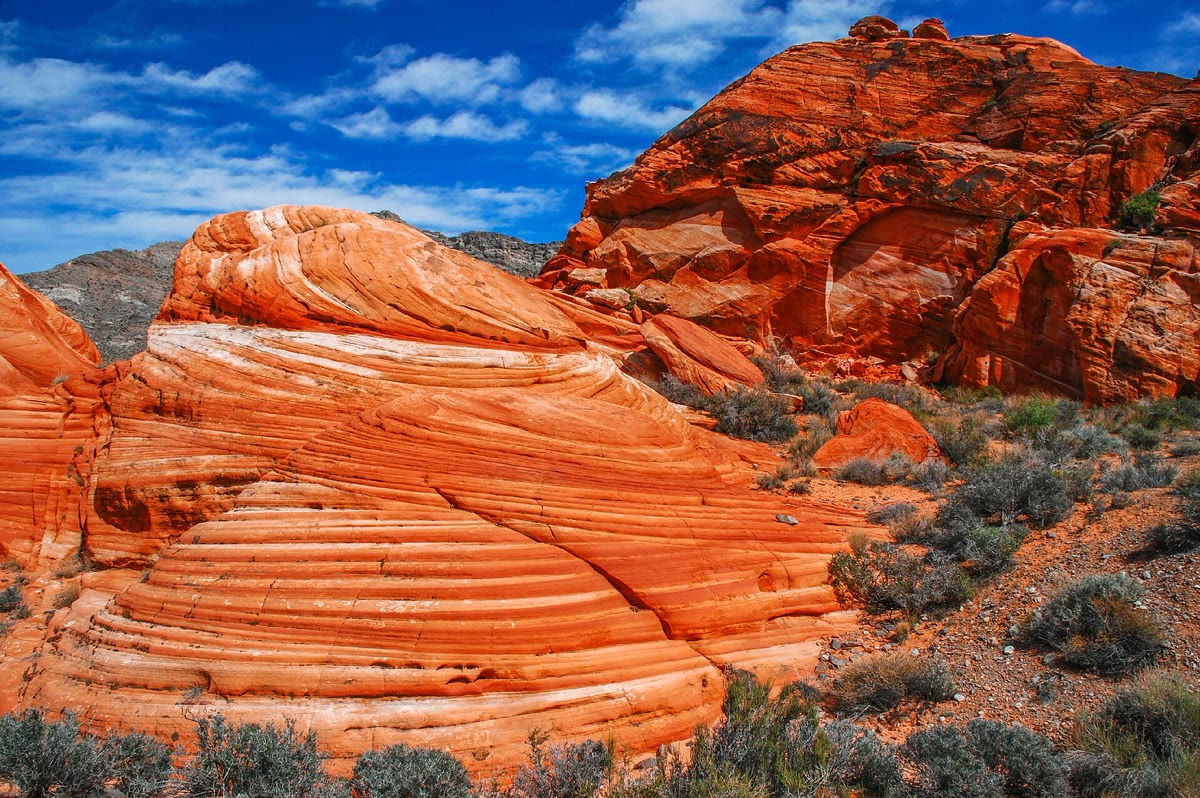
\includegraphics[height=3.6cm]{images/book3/b1-cross-bedding-aztec.jpg}};
\end{tikzpicture}

{\small Left: the geometry of climbing \omterm{def:b1:clastic-sediments:bedform}{bedforms} (schematic, angles exaggerated).
The troughs travel along straight paths inclined at the angle of climb $\theta$
(thick lines); between two of them the lower parts of the foresets are
preserved, in sets of thickness $T = L\sin\theta$. Right: \omterm{def:b1:clastic-sediments:cross-bedding}{cross-bedding} in the
Aztec Sandstone, Muddy Mountains, Nevada: inclined sets of laminae, each cut off
at the top by the erosion surface at the base of the next. Photograph Chip
Carroon, Bureau of Land Management, CC~BY-SA~2.0, via Wikimedia Commons.}
\label{fig:b1:clastic-sediments:climb}
\end{omfigure}
% ledger: southard:climb, commons:aztec-crossbed

\emph{\omterm{def:b1:clastic-sediments:cross-bedding}{Palaeocurrents}.} The \omterm{def:b1:geological-maps:attitude}{dip directions} of cross-beds measured on an \omterm{def:b1:geological-maps:geological-map}{outcrop}
scatter around the mean direction of the current, because the lee faces of
\omterm{def:b1:clastic-sediments:bedform}{dunes} and \omterm{def:b1:clastic-sediments:bedform}{ripples} are curved and the currents themselves wander. Their mean is
taken as a vector mean, not an arithmetic one, for the reason shown in
\cref{prop:b1:field-lab-methods-1:vector-mean}: \omterm{def:b1:spherical-astronomy:horizontal}{azimuths} are angles on a
circle, and 350 and 010 average to 000, not 180.

\begin{proposition}[Mean of azimuths]\label{prop:b1:clastic-sediments:azimuths}
Let $\alpha_1, \ldots, \alpha_N$ be \omterm{def:b1:spherical-astronomy:horizontal}{azimuths}, measured clockwise from north.
Their vector mean $\bar\alpha$ and their mean resultant length $\bar R$ are
given by
\[
  S = \sum_{i=1}^N \sin\alpha_i, \quad C = \sum_{i=1}^N \cos\alpha_i, \quad
  \bar\alpha = \operatorname{atan2}(S, C), \quad \bar R = \frac{\sqrt{S^2 + C^2}}{N},
\]
where $\operatorname{atan2}(S, C)$ is the angle whose sine and cosine are
proportional to $S$ and $C$, taken between \ang{0} and \ang{360}. $\bar R$ lies
between 0 and 1, and is 1 only if all the \omterm{def:b1:spherical-astronomy:horizontal}{azimuths} are equal.
\end{proposition}

\begin{proof}
The unit vector of \omterm{def:b1:spherical-astronomy:horizontal}{azimuth} $\alpha$, with east as the first coordinate and north
as the second, is $(\sin\alpha, \cos\alpha)$. The sum of the $N$ unit vectors is
$(S, C)$, and its direction, the vector mean
(\cref{def:b1:field-lab-methods-1:mean-orientation}), has the \omterm{def:b1:spherical-astronomy:horizontal}{azimuth} whose
sine and cosine are $S/\sqrt{S^2+C^2}$ and $C/\sqrt{S^2+C^2}$. By the triangle
inequality the length of a sum of $N$ unit vectors is at most $N$, with equality
only when they all point the same way.
\end{proof}

\begin{method}[Palaeocurrent from cross-bedding]\label{met:b1:clastic-sediments:palaeocurrent}
\begin{enumerate}
  \item On each set, measure the \omterm{def:b1:geological-maps:attitude}{dip direction} of the foresets, choosing
        surfaces that show their true \omterm{def:b1:geological-maps:attitude}{dip} (or measure \omterm{def:b1:geological-maps:attitude}{strike} and \omterm{def:b1:geological-maps:attitude}{dip}).
  \item Measure the \omterm{def:b1:geological-maps:attitude}{attitude} of the main bedding; if it is tilted by more than a
        few degrees, rotate each foreset back to the horizontal about the \omterm{def:b1:geological-maps:attitude}{strike}
        of the bedding (a rotation done with the stereographic projection of the Year~3 volume).
  \item Compute the vector mean $\bar\alpha$ and $\bar R$ of the corrected \omterm{def:b1:geological-maps:attitude}{dip
        directions} (\cref{prop:b1:clastic-sediments:azimuths}).
  \item Plot the readings as a rose diagram, a circular histogram of \omterm{def:b1:spherical-astronomy:horizontal}{azimuths},
        to see whether they form one group or two: tidal currents that reverse
        build sets that \omterm{def:b1:geological-maps:attitude}{dip} in opposite directions, in herringbone
        \omterm{def:b1:clastic-sediments:cross-bedding}{cross-bedding}, and a single mean is then meaningless.
\end{enumerate}
\end{method}
% ledger: og:sorting-environments

\emph{Other structures.} Several other structures record the conditions of
deposition and the way up of the beds. A \omterm{def:b1:clastic-sediments:turbidite}{graded bed} fines upward, from coarse at
its base to fine at its top, as grains settle from a waning current, the
coarsest first (\cref{def:b1:clastic-sediments:turbidite}). Mud cracks, polygons
of shrinkage cracks filled by the next layer, form where mud dries in the air,
as on tidal flats and floodplains. Scours cut by the current into the mud
below, and filled by the sand above, are preserved as casts on the base of the
sandstone bed, and their shapes point the way the current went.
% ledger: og:sorting-environments

\section{Facies, rivers and deltas}\label{sec:b1:clastic-sediments:rivers-deltas}

Grain size, \omterm{def:b1:clastic-sediments:sorting}{sorting}, structures, fossils and composition together make the
character of a sedimentary rock, and geologists use one word for that
character.

\begin{definition}[Sedimentary facies, depositional environment]\label{def:b1:clastic-sediments:facies}
A \emph{sedimentary facies}\index{sedimentary facies} is a body of sedimentary
rock distinguished from others by its lithology, grain size, sedimentary
structures and fossils, all of which reflect the conditions under which it was
formed. The \emph{depositional environment}\index{depositional environment} is
the place, with its physical, chemical and biological conditions, in which a
sediment is laid down: a river channel, a floodplain, a beach, the slope of a
delta, the deep sea floor.
\end{definition}
% ledger: og:sorting-environments

A facies is a description, an environment an interpretation, and several
environments can make the same facies: rippled sand is laid down in rivers, on
tidal flats and on the deep sea floor. The interpretation therefore rests on
associations of facies and on the order in which they are stacked, which follow
the movement of the environments in space: the general laws of that stacking,
and the standard models of each environment, are the subject of the Year~3
volume. This chapter describes the main clastic environments and the vertical
successions that identify them.

\emph{Braided and meandering rivers.} Rivers come in two main styles. A braided
river flows in many channels that split and rejoin around bars of gravel and
sand; braided rivers carry coarse loads near their sources, below mountains or
in front of glaciers, and their deposits are sheets of gravel and coarse,
cross-bedded sand, with little mud. A meandering river flows in a single
sinuous channel. The fastest water runs along the outside of each bend, where
it erodes the cut bank; on the inside, where the water is slowest, sand is laid
down on the point bar. The meander thus migrates sideways, eroding on one side
and building on the other; the floodplain beyond the banks receives only the
mud of the floods.
% ledger: og:rivers

The succession of the point bar follows from the \omterm{def:b1:clastic-sediments:bedform}{bedforms}. At the foot of the
bar, in the deepest and fastest water, the current leaves the coarsest grains
and builds \omterm{def:b1:clastic-sediments:bedform}{dunes}; up the gently sloping bar the water becomes shallower and
slower, the sand finer and the \omterm{def:b1:clastic-sediments:bedform}{dunes} give way to \omterm{def:b1:clastic-sediments:bedform}{ripples}
(\cref{sec:b1:clastic-sediments:bedforms}); at the top, the bar passes into
the floodplain. As the bend migrates, each of these zones moves over the one
below it, and a borehole through the deposit meets them stacked: a fining-upward
succession from an erosion surface to mud, one for each passage of a channel,
whose thickness is about the depth of the channel that made it.

\emph{Deltas.} Where a river enters a standing body of water, its current
spreads and slows, and its load is dropped: the coarse load near the mouth, the
fine load farther out. A delta grows forward, or progrades, as long as the
river supplies more sediment than the waves and tides can carry away. What the
waves and the tides do to the supply decides its shape.

\begin{definition}[River-, wave- and tide-dominated deltas]\label{def:b1:clastic-sediments:delta}
A delta is \emph{river-dominated}\index{river-dominated delta} when the river's
supply overwhelms the waves and tides, and its distributary channels, confined by
their own levees, build long fingers of sand into the sea; it is
\emph{wave-dominated}\index{wave-dominated delta} when waves rework the sand
brought to the mouths into beaches and beach ridges along a smooth, arched
coast; it is \emph{tide-dominated}\index{tide-dominated delta} when tidal
currents, flowing in and out of the mouths, shape its sand into bars and ridges
parallel to the flow, separated by funnel-shaped channels.
\end{definition}
% ledger: og:deltas

\begin{omfigure}
\begin{tikzpicture}[font=\footnotesize, >={Stealth[length=4pt]}]
% meander in plan view (schematic) and the fining-upward log of a point bar
\begin{scope}[yscale=0.8]
  \fill[green!8] (-0.2,-0.4) rectangle (7.2,4.4);
  \draw[omSea!80!black, line width=9pt] plot[smooth, tension=0.7] coordinates {(0,3.6) (1.4,3.7) (2.6,2.8) (2.3,1.4) (3.2,0.5) (4.6,0.8) (5.0,2.2) (5.6,3.4) (7.0,3.5)};
  \draw[omSea!45, line width=7pt] plot[smooth, tension=0.7] coordinates {(0,3.6) (1.4,3.7) (2.6,2.8) (2.3,1.4) (3.2,0.5) (4.6,0.8) (5.0,2.2) (5.6,3.4) (7.0,3.5)};
  % point bars (inside of bends) with scroll lines
  \foreach \r in {0.25,0.45,0.65} {\draw[brown!60!black, densely dotted] (3.45,1.15) ++(200:\r) arc[start angle=200, end angle=340, radius=\r];}
  \fill[brown!25, opacity=0.8] (3.45,1.25) ellipse[x radius=0.55, y radius=0.35];
  \node[align=center] at (3.45,1.95) {point bar\\ (deposition)};
  \fill[brown!25, opacity=0.8] (1.75,2.75) ellipse[x radius=0.4, y radius=0.45];
  \node[align=center] at (1.3,1.95) {point bar};
  \draw[red!60!black, thick] (2.9,0.2) .. controls (3.3,0.0) and (4.3,0.15) .. (4.85,0.6);
  \node[red!60!black, anchor=north] at (4.0,0.0) {cut bank (erosion)};
  \draw[->, black!70] (5.9,3.0) -- (6.7,3.15) node[right] {flow};
  \node[anchor=north west, black!60] at (5.2,1.3) {floodplain};
  \node[font=\footnotesize] at (3.5,-0.85) {(a) a meander, in plan view};
\end{scope}
\begin{scope}[xshift=9.2cm, yshift=-0.3cm, yscale=0.8]
  % log: x width = grain size; y = height
  \draw[lith shale] (0,3.6) rectangle (0.8,4.6);
  \draw[lith sandstone] (0,2.6) rectangle (1.2,3.6);
  \draw[lith sandstone] (0,0.6) rectangle (1.7,2.6);
  \draw[lith conglomerate] (0,0) rectangle (2.2,0.6);
  \draw[very thick, red!60!black] (0,0) -- (2.2,0);
  % cross-bed symbols
  \foreach \y in {0.9,1.5,2.1} {\draw[black!70] (0.3,\y) .. controls (0.6,\y+0.05) and (0.9,\y+0.25) .. (1.2,\y+0.4);}
  \foreach \x in {0.2,0.5,0.8} {\draw[black!70] (\x,3.0) -- ++(0.12,0.1) -- ++(0.12,-0.1);}
  \node[anchor=west, align=left] at (2.4,4.1) {floodplain mud,\\ roots, mud cracks};
  \node[anchor=west, align=left] at (2.4,3.1) {fine sand, ripple\\ cross-lamination};
  \node[anchor=west, align=left] at (2.4,1.6) {medium to coarse sand,\\ dune cross-bedding};
  \node[anchor=west, align=left] at (2.4,0.3) {gravel lag on an\\ erosion surface};
  \draw[->] (-0.35,0) -- (-0.35,4.6) node[above] {up};
  \draw[<->, black!60] (-0.7,0) -- node[above, rotate=90, font=\scriptsize] {channel depth} (-0.7,3.6);
  \node[font=\footnotesize] at (1.8,-0.5) {(b) point-bar succession};
\end{scope}
\end{tikzpicture}

{\small (a)~A meandering river (schematic): the current erodes the outer bank of
each bend and lays sand on the point bar inside it; the curved scroll lines are
the bar's successive positions. (b)~The succession left by a migrating point
bar, the width of each layer proportional to its grain size (schematic). It
fines upward, and its thickness records the depth of the channel.}
\label{fig:b1:clastic-sediments:point-bar}
\end{omfigure}
% ledger: og:rivers, southard:phase-diagram

The three end members are the corners of a triangle in which any delta can be
placed by the relative strength of the three processes. The bird's-foot delta of
the Mississippi, with its long fingers into the Gulf of Mexico
(\cref{ch:b1:erosion-transport}), is the classic \omterm{def:b1:clastic-sediments:delta}{river-dominated delta}; the
Nile, with its smooth arc of beaches, a \omterm{def:b1:clastic-sediments:delta}{wave-dominated} one; the delta of the
Ganges and Brahmaputra, the largest in the world, a \omterm{def:b1:clastic-sediments:delta}{tide-dominated} one.
% ledger: og:deltas

\begin{omfigure}
\begin{tikzpicture}[font=\footnotesize]
% delta classification triangle (schematic) and the Lena delta from Landsat
\begin{scope}[yscale=0.82]
  \coordinate (R) at (2.6,4.5); \coordinate (W) at (0,0); \coordinate (T) at (5.2,0);
  \fill[omDef!8] (R) -- (W) -- (T) -- cycle;
  \draw[thick] (R) -- (W) -- (T) -- cycle;
  \node[above, align=center] at (R) {\textbf{river-dominated}\\ elongate fingers, levees};
  \node[below, align=center] at (W) {\textbf{wave-dominated}\\ smooth beach ridges};
  \node[below, align=center] at (T) {\textbf{tide-dominated}\\ bars along the flow};
  \fill[omThm] (2.6,2.9) circle[radius=2pt] node[below=1pt] {Mississippi};
  \fill[omThm] (0.75,0.4) circle[radius=2pt] node[above right=0pt] {Nile};
  \fill[omThm] (4.4,0.4) circle[radius=2pt] node[above left=0pt, align=right] {Ganges--\\ Brahmaputra};
\end{scope}
\node[anchor=south west, inner sep=0] at (7.2,-0.9) {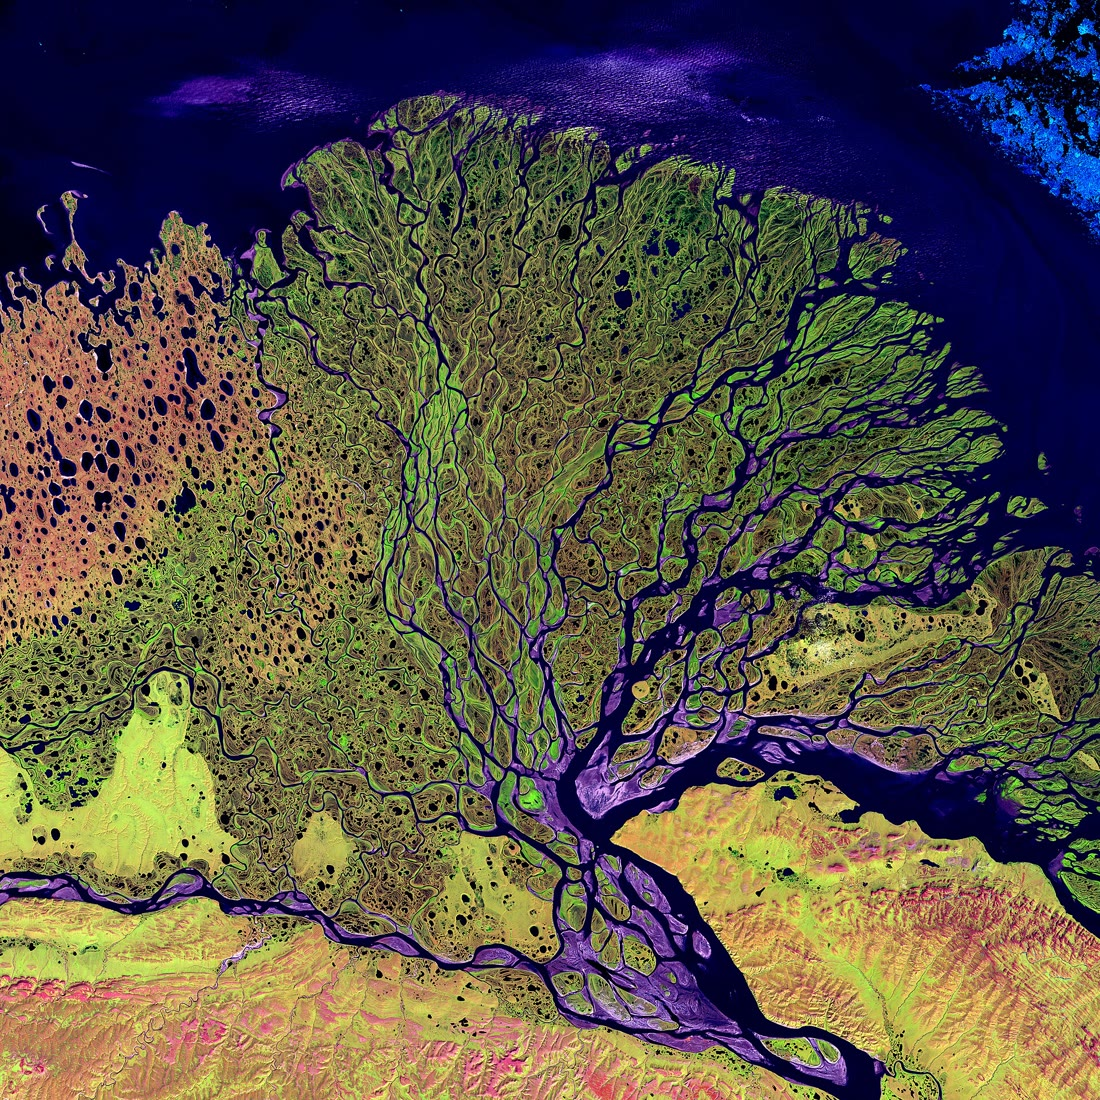
\includegraphics[height=5.2cm]{images/book3/b1-lena-delta.jpg}};
\end{tikzpicture}

{\small Left: the three end members of deltas, after the process that shapes
them (schematic; the positions of the three examples are indicative). Right:
the delta of the Lena, in Siberia, built into the Laptev Sea (top); the river
enters from the bottom right and splits into hundreds of distributaries. Landsat~7
false-colour image of 27~February 2000, U.S. Geological Survey, public domain,
via Wikimedia Commons.}
\label{fig:b1:clastic-sediments:deltas}
\end{omfigure}
% ledger: og:deltas, commons:lena-delta

\emph{The coarsening-upward succession.} In front of the river mouth, the
delta has a gently sloping front, the delta front, which passes seaward into the
prodelta, where only mud settles from suspension. As the delta progrades, each
of these zones advances over the one in front of it: a borehole on the delta
plain meets, from bottom to top, the laminated muds of the prodelta, then
alternating silt and sand of the lower delta front, then the cross-bedded sand
of the mouth bars, cut at the top by the channels of the delta plain. The
succession coarsens upward, the reverse of a point bar, and its thickness is
about the depth of water into which the delta built. Its rate is linked to the
geometry of the delta front.

\begin{proposition}[Progradation and accumulation]\label{prop:b1:clastic-sediments:progradation}
Let a delta front of constant slope $\alpha$ advance horizontally at the speed
$v$ without changing shape, at constant sea level. A fixed point under the front
then receives sediment at the vertical rate
\[
  a = v\,\tan\alpha,
\]
and the delta-front succession of thickness $h$ accumulates there in the time
$h/(v\tan\alpha)$.
\end{proposition}

\begin{proof}
In the time $\mathrm dt$ the front moves forward by $v\,\mathrm dt$. At a fixed
point under the sloping surface, the surface rises by the difference of
height between two points of the front a horizontal distance $v\,\mathrm dt$
apart, that is $v\,\mathrm dt\,\tan\alpha$, hence the rate. The front crosses
the point while the surface rises by $h$, which takes the time $h/a$.
\end{proof}

Delta fronts slope gently, so $\tan\alpha$ is small: the front of a delta
advances far faster than the sediment piles up at any point under it
(\cref{exo:b1:clastic-sediments:12}).

\begin{inthelab}[Describing a core]
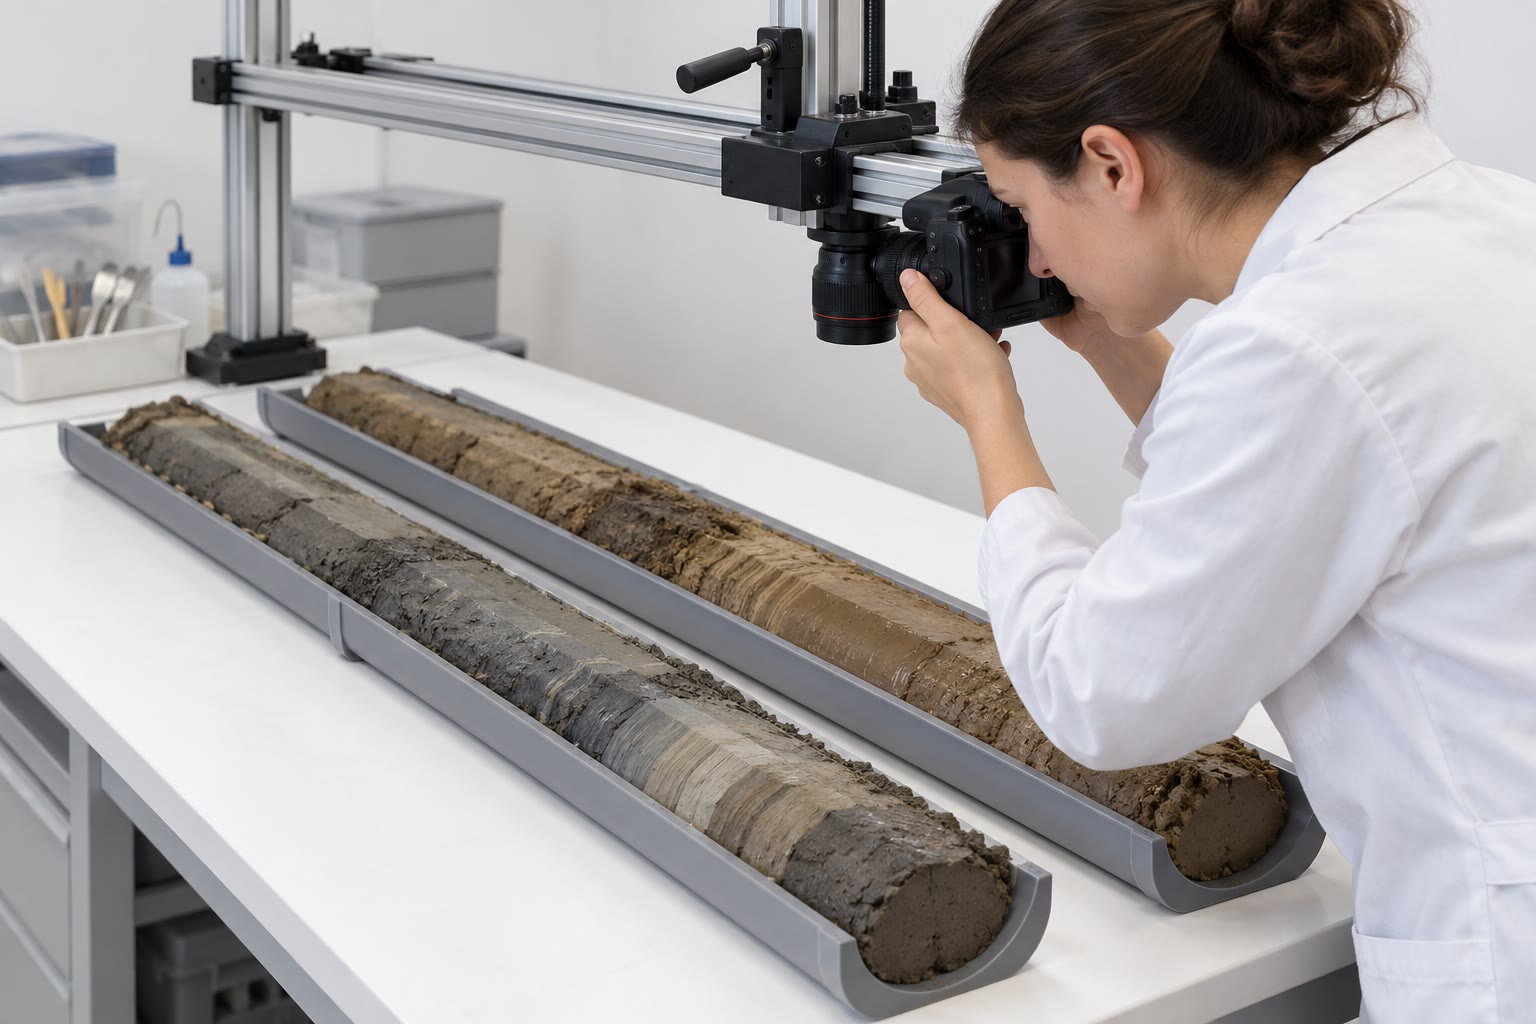
\includegraphics[width=0.3\linewidth]{images/book3/ai/b1-core-lab.jpg}\hfill
\begin{minipage}[b]{0.67\linewidth}
The cylinders of sediment or rock brought up by a drill are laid in trays in
the order of depth, split lengthwise, and photographed under even light before
they dry and change colour. The sedimentologist then draws a log of the core,
metre by metre: the lithology, the grain size of each bed (the width of the
column), the structures (\omterm{def:b1:clastic-sediments:cross-bedding}{cross-bedding}, lamination, grading, burrows), the
\omterm{def:b1:geological-maps:geological-map}{contacts}, sharp or gradual, the colour and the fossils. Samples are taken for
grain-size analysis and \omterm{def:b1:field-lab-methods-1:thin-section}{thin sections}. A core is a single narrow window: the
direction of the cross-beds is lost unless the core was oriented, and the
lateral extent of the beds must come from other boreholes.
\end{minipage}

\smallskip
{\small A core laid out to be photographed in a sediment laboratory (AI
illustration).}
\end{inthelab}

\section{Shoreline and shelf}\label{sec:b1:clastic-sediments:shoreline}

Along the coast between the deltas, the sand brought by the rivers is shaped by
waves and tides. A beach is sand reworked by the swash, the thin sheet of water
that runs up and down it after each wave breaks: the grains are moved again and
again, the fine ones are carried offshore, and beach sands are among the best
sorted and most rounded of all sediments. Their laminae, laid down by the
swash, \omterm{def:b1:geological-maps:attitude}{dip} gently seaward. On many low coasts the sand forms barrier islands,
long ridges of beach and wind-blown \omterm{def:b1:clastic-sediments:bedform}{dunes} separated from the mainland by
lagoons, which are quiet and fine-grained, connected to the sea by tidal
inlets.

Where the tides are strong and the waves weak, the coast is fringed by tidal
flats, covered and uncovered twice a day. They grade from sand near the low-tide
line, where the currents are strongest, to mud near the high-tide line, where
the slack water lets clay settle; their deposits show the reversing flow in
herringbone \omterm{def:b1:clastic-sediments:cross-bedding}{cross-bedding}, the drying in mud cracks, and the alternation of
current and slack water in thin draped layers of mud on rippled sand.

Offshore, the shelf is swept by waves only down to a depth that grows with the
size of the waves. Above it sand is winnowed and moved; below it mud settles,
except during storms, when the larger waves reach deeper and lay down sheets of
sand with the gentle undulating lamination called hummocky cross-stratification.
A shelf succession thus often alternates fair-weather mud with storm sands, the
thicker and coarser toward the shore.
% ledger: og:sorting-environments, folk:maturity

\section{Deep-sea clastics}\label{sec:b1:clastic-sediments:deep-sea}

Sand and gravel also reach the floors of the deep oceans, thousands of metres
down and hundreds of kilometres from land, and they are carried there by flows
that no one has seen in full: dense, sediment-laden currents running down the
continental slope under the clear water of the ocean.

\begin{history}[Cables on the sea floor, 1929]
On 18~November 1929 an earthquake of \omterm{def:b1:earthquake-source:mw}{moment magnitude} 7.2 struck the continental
slope south of Newfoundland, along the southern edge of the Grand Banks. A slump
of some \qty{200}{km^3} of sediment moved on the slope, and a tsunami killed 28
people on the coast of Newfoundland. Twelve telegraph cables laid across the
sea floor broke, some in several places. Those near the epicentre broke at once;
the others, farther south and deeper, broke one after another in the following
hours, in order of distance down the slope. In 1952 Bruce Heezen and Maurice Ewing,
studying the times of the breaks, explained them: the slump had turned into a
\omterm{def:b1:clastic-sediments:turbidite}{turbidity current} that ran down the slope and out across the abyssal plain for
more than 480 miles, breaking each cable as it passed. From the times and
distances they estimated its speed at about 50 knots on the upper continental
rise, where the slope is about \qty{0.5}{\percent}, and still 12 knots at the
last cable, about 400 miles from its origin. As it slowed, they argued, it must
have laid down a \omterm{def:b1:clastic-sediments:turbidite}{graded bed} over the plain, finer and finer upward.
\end{history}
% ledger: nrcan:grand-banks, he52:grand-banks

Fifty knots is \qty{25.7}{m.s^{-1}}, over \qty{90}{km.h^{-1}}, the speed of a
car on a main road; 12 knots is \qty{6.2}{m.s^{-1}}; and 480 miles are about
\qty{770}{km}. The breaks also gave the first measured speeds of a flow that
had been inferred only from its deposits and from experiments in tanks.
% ledger: he52:grand-banks

\begin{definition}[Turbidity current, turbidite, graded bed]\label{def:b1:clastic-sediments:turbidite}
A \emph{turbidity current}\index{turbidity current} is a current of water made
denser than the water around it by the sediment it holds in suspension, which
flows down a slope under that water, its grains kept in suspension by the
turbulence that its own motion creates. A \emph{turbidite}\index{turbidite} is
the deposit of a turbidity current. A \emph{graded bed}\index{graded bed} is a
bed whose grain size decreases from its base to its top.
\end{definition}
% ledger: og:sorting-environments, he52:grand-banks

A \omterm{def:b1:clastic-sediments:turbidite}{turbidity current} drives itself: it runs because its suspension is heavy, and
it keeps its suspension because it runs. On a steep slope it can pick up more
sediment from the bed, become denser and accelerate; on the gentle slope of the
abyssal plain it slows, drops its load and dies.

\begin{proposition}[Speed of a turbidity current]\label{prop:b1:clastic-sediments:turbidity}
A \omterm{def:b1:clastic-sediments:turbidite}{turbidity current} of thickness $h$ and density $\rho + \Delta\rho$ flows
steadily down a slope $S$ under water of density $\rho$. If the resistance of
the bed and of the water above is $\tau = \rho\,C_f\,U^2$ per unit area, $C_f$
being a dimensionless friction coefficient, its mean speed is
\[
  U = \sqrt{\frac{\Delta\rho}{\rho}\,\frac{g\,h\,S}{C_f}} .
\]
\end{proposition}

\begin{proof}
The argument is that of the depth--slope product
(\cref{prop:b1:erosion-transport:depth-slope}), with the weight replaced by
the excess weight. A column of the current of unit area weighs $(\rho +
\Delta\rho) g h$, and the water it displaces $\rho g h$: in the surrounding
water, only the excess $\Delta\rho\,g\,h$ pulls it down the slope, with the
component $\Delta\rho\,g\,h\,S$ along it. In steady flow this balances the
resistance $\rho C_f U^2$, hence $U^2 = (\Delta\rho/\rho)\,g\,h\,S/C_f$.
\end{proof}

The resistance law $\tau = \rho C_f U^2$, quadratic in the speed, is the one of
turbulent flows in hydraulics (the physics books), and $C_f$ is found by
experiment. The formula neglects the water that the current mixes into
itself through its upper surface, which dilutes and slows it. It shows the role
of the three factors: a current twice as thick, or twice as dense, or on a slope
twice as steep, runs $\sqrt 2$ times faster. A suspension holding the
fraction $c$ of its volume as quartz grains has $\Delta\rho/\rho = 1.65\,c$
(\cref{sec:b1:erosion-transport:settling}), small unless the flow is very
concentrated; this is where a \omterm{def:b1:clastic-sediments:turbidite}{turbidity current} differs from a river, in which
the whole weight of the water, not a small excess, drives the flow. To run at the 50 knots of 1929 on a slope of half a per cent,
a \omterm{def:b1:clastic-sediments:turbidite}{turbidity current} needs a large product of thickness and density excess
(\cref{exo:b1:clastic-sediments:11}).

\emph{The Bouma sequence.} In 1962 Arnold Bouma described the internal order of
the sandstone beds of ancient deep-sea successions in five divisions, labelled
from the base up. A: massive or graded sand, often on an erosive base; B: sand
with parallel lamination; C: fine sand with \omterm{def:b1:clastic-sediments:bedform}{ripple} cross-lamination, often
convolute; D: laminated silt grading into mud; E: mud. The order is read as the
record of a single waning current passing over a point: as it slows, it drops
first its coarsest grains en masse, then builds an upper plane bed, then
\omterm{def:b1:clastic-sediments:bedform}{ripples}, then lets the silt and clay settle. Complete sequences are rare: the
upper divisions are often eroded by the next current, and far from the source,
where the current is weak, the lower ones are missing.
% ledger: og:sorting-environments, shanmugam:bouma

\begin{omfigure}
\begin{tikzpicture}[font=\footnotesize]
% Bouma sequence: log (schematic) and a labelled photograph
\begin{scope}
  \draw[lith shale] (0,4.0) rectangle (0.7,4.8);
  \draw[lith shale] (0,3.3) rectangle (0.9,4.0);
  \draw[lith sandstone] (0,2.2) rectangle (1.3,3.3);
  \draw[lith sandstone] (0,1.2) rectangle (1.6,2.2);
  \draw[lith sandstone] (0,0) rectangle (2.0,1.2);
  \draw[very thick, red!60!black] (0,0) .. controls (0.6,-0.12) and (1.4,0.1) .. (2.0,0);
  \foreach \y in {1.4,1.6,1.8,2.0} {\draw[black!70] (0.1,\y) -- (1.5,\y);}
  \foreach \x in {0.15,0.5,0.85} {\draw[black!70] (\x,2.55) .. controls (\x+0.12,2.75) .. (\x+0.3,2.6);}
  \foreach \y in {3.45,3.6,3.75,3.9} {\draw[black!60] (0.1,\y) -- (0.8,\y);}
  \foreach \x/\y in {0.4/0.3, 0.9/0.5, 1.4/0.25, 0.6/0.8, 1.2/0.9} {\fill[black!60] (\x,\y) circle[radius=0.06];}
  \node[anchor=west] at (2.2,4.4) {E \quad mud};
  \node[anchor=west] at (2.2,3.65) {D \quad laminated silt to mud};
  \node[anchor=west] at (2.2,2.75) {C \quad ripple cross-lamination};
  \node[anchor=west] at (2.2,1.7) {B \quad parallel lamination};
  \node[anchor=west] at (2.2,0.6) {A \quad graded sand};
  \node[anchor=west, red!60!black] at (2.2,-0.15) {erosive base, sole marks};
  \draw[->] (-0.3,0) -- (-0.3,4.8) node[above] {up};
\end{scope}
\node[anchor=south west, inner sep=0] at (6.9,-0.3) {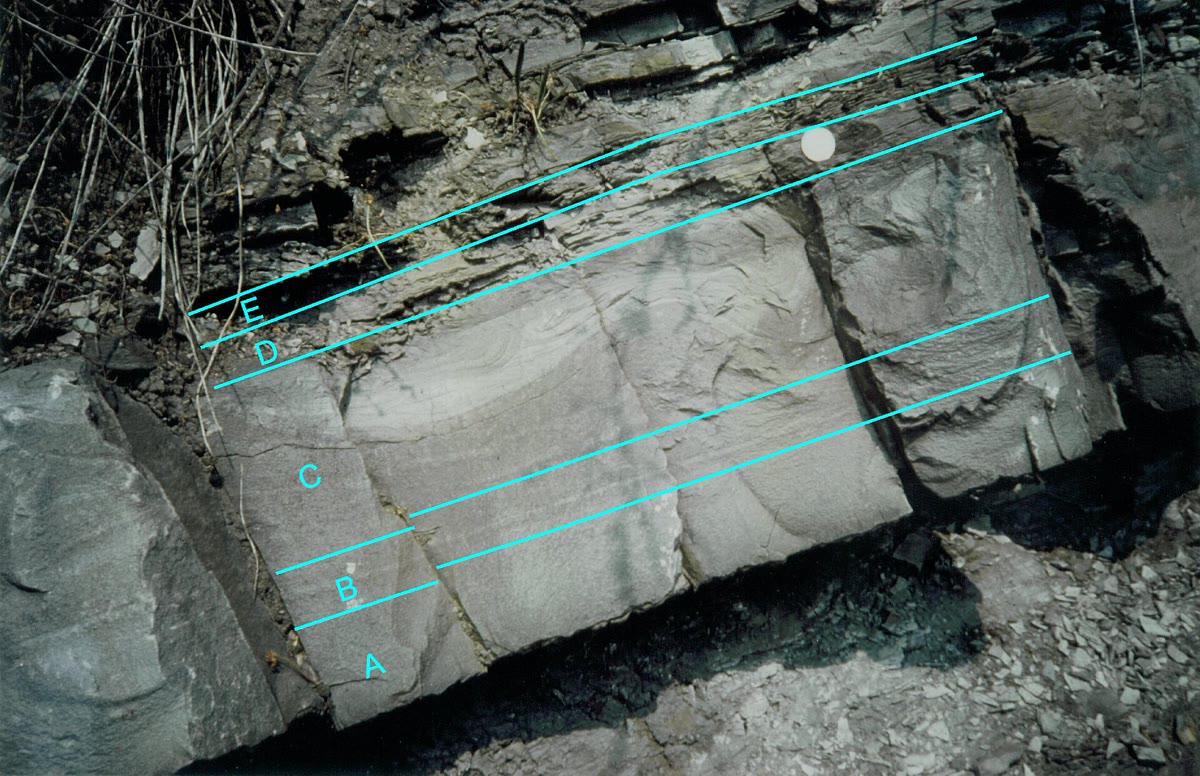
\includegraphics[height=5.2cm]{images/book3/b1-turbidite-bouma.jpg}};
\end{tikzpicture}

{\small Left: the five divisions of the Bouma sequence, the width of each
proportional to its grain size (schematic). Right: a \omterm{def:b1:clastic-sediments:turbidite}{turbidite} bed of the Upper
Devonian at Becke-Oese, Germany, with the divisions A to E marked by the
photographer; the coin gives the scale. Photograph Jo Weber, CC~BY-SA~3.0, via
Wikimedia Commons.}
\label{fig:b1:clastic-sediments:bouma}
\end{omfigure}
% ledger: og:sorting-environments, shanmugam:bouma, commons:bouma-becke-oese

The Bouma sequence became the standard model of the \omterm{def:b1:clastic-sediments:turbidite}{turbidite}, and thousands of
ancient deep-sea sandstones were interpreted with it. The interpretation is
disputed: currents running along the slope, deep tidal currents and internal
waves also build rippled and laminated sands, and some sedimentologists argue
that many beds read as \omterm{def:b1:clastic-sediments:turbidite}{turbidites}, including some of those of the type area,
were laid down by other flows. Few \omterm{def:b1:clastic-sediments:turbidite}{turbidity currents} have been observed in the
modern ocean, while ancient \omterm{def:b1:clastic-sediments:turbidite}{turbidites} are counted by the thousands.
% ledger: shanmugam:bouma

Not all deep-sea clastics are \omterm{def:b1:clastic-sediments:turbidite}{turbidites}. Contour currents, the slow, deep
currents that follow the contours of the continental slope, rework the sediment
of the slope into smooth, elongated drifts, the contourites. And far from the
continents, where neither \omterm{def:b1:clastic-sediments:turbidite}{turbidity currents} nor contour currents reach, the
sea floor receives only what settles from the water above: the shells of
plankton and the finest windblown dust, the pelagic sediments of the next
chapter (\cref{ch:b1:chemical-biogenic-sediments}).
% ledger: og:sorting-environments

\section{Exercises}

\begin{exercise}[$\star$]\label{exo:b1:clastic-sediments:1}
Convert to phi units the diameters \qty{0.18}{mm}, \qty{0.75}{mm},
\qty{3}{mm}, \qty{0.012}{mm} and \qty{150}{mm}, to two decimals, and name the
class of each (\cref{tab:b1:clastic-sediments:classes}).
% ledger: folk:wentworth-classes
\end{exercise}

\begin{exercise}[$\star$]\label{exo:b1:clastic-sediments:2}
The cumulative curve of a river sand gives $\varphi_5 = 0.62$, $\varphi_{16} =
1.05$, $\varphi_{50} = 1.71$, $\varphi_{84} = 2.43$ and $\varphi_{95} = 2.98$.
Compute its graphic mean, in phi units and in millimetres, and its inclusive
graphic standard deviation, and name its size and its \omterm{def:b1:clastic-sediments:sorting}{sorting}.
% ledger: folk:graphic-measures, folk:sorting-classes
\end{exercise}

\begin{exercise}[$\star$]\label{exo:b1:clastic-sediments:3}
\omterm{def:b1:clastic-sediments:bedform}{Ripples} \qty{2}{cm} high migrate at \qty{1}{cm} a minute over a bed of quartz
sand of porosity \num{0.4}. With \cref{prop:b1:clastic-sediments:migration},
compute the volume of \omterm{def:b1:erosion-transport:load}{bed load} per unit width, in \si{m^2.s^{-1}}, and the mass
of quartz ($\qty{2650}{kg.m^{-3}}$) carried over a metre of crest in a day.
% ledger: hom:quartz
\end{exercise}

\begin{exercise}[$\star$]\label{exo:b1:clastic-sediments:4}
A knot is one nautical mile, \qty{1852}{m}, per hour. (a)~Convert to metres
per second the speeds of 50 and 12 knots estimated for the \omterm{def:b1:clastic-sediments:turbidite}{turbidity current} of
1929. (b)~How long does a current at 12 knots take to cover \qty{100}{km}?
(c)~Convert 480 and 400 miles to kilometres (one mile is \qty{1.609}{km}).
% ledger: he52:grand-banks
\end{exercise}

\begin{exercise}[$\star\star$]\label{exo:b1:clastic-sediments:5}
(a)~Using the percentiles of a normal distribution given in the proof of
\cref{prop:b1:clastic-sediments:normal}, compute the graphic standard
deviation $(\varphi_{84} - \varphi_{16})/2$ and the estimate
$(\varphi_{95} - \varphi_5)/3.3$ for a normal distribution of standard
deviation $\sigma$. (b)~Why might the two disagree for a real sediment? Which
kind of sediment makes them differ the most?
\end{exercise}

\begin{exercise}[$\star\star$]\label{exo:b1:clastic-sediments:6}
A deposit of climbing \omterm{def:b1:clastic-sediments:bedform}{ripples} shows sets \qty{1.5}{cm} thick, measured
perpendicular to their boundaries, made by \omterm{def:b1:clastic-sediments:bedform}{ripples} spaced at \qty{15}{cm}.
(a)~Compute the angle of climb. (b)~If the \omterm{def:b1:clastic-sediments:bedform}{ripples} moved at
\qty{0.5}{cm} a minute, at what rate was the bed raised, in centimetres per
hour? (c)~What does such a rate say about the flow?
% ledger: southard:climb
\end{exercise}

\begin{exercise}[$\star\star$]\label{exo:b1:clastic-sediments:7}
Six cross-bed \omterm{def:b1:geological-maps:attitude}{dip directions}, already corrected for the tilt of the beds,
read 350, 020, 005, 340, 015 and 030. (a)~Compute their arithmetic mean. (b)~Compute
their vector mean and $\bar R$. (c)~Explain the difference.
\end{exercise}

\begin{exercise}[$\star\star$]\label{exo:b1:clastic-sediments:8}
Three sandstones are examined in \omterm{def:b1:field-lab-methods-1:thin-section}{thin section}. A has \qty{12}{\percent} of
clay matrix and angular grains of quartz, \omterm{def:b1:rock-forming-minerals:groups}{feldspar} and rock fragments. B has
\qty{2}{\percent} of clay, $\sigma_I = 0.40\,\varphi$ and quartz grains of
roundness \num{2.2} on Folk's scale. C has no clay, $\sigma_I =
0.30\,\varphi$, quartz grains of roundness \num{3.6}, and \qty{98}{\percent}
quartz. Name the \omterm{def:b1:clastic-sediments:maturity}{textural maturity} of each, and suggest an environment of
deposition for each.
% ledger: folk:maturity
\end{exercise}

\begin{exercise}[$\star\star$]\label{exo:b1:clastic-sediments:9}
(a)~Compute the Froude number of a flow \qty{0.3}{m} deep at
\qty{1.5}{m.s^{-1}}, and of a river \qty{2}{m} deep at \qty{1.0}{m.s^{-1}} ($g
= \qty{9.81}{m.s^{-2}}$). (b)~At what depth would a flow of
\qty{1.5}{m.s^{-1}} reach a Froude number of 1, and what speed would the river
\qty{2}{m} deep need? (c)~Why are antidunes common in sheets of water running
off a beach, and rare in large rivers?
% ledger: southard:ripples-dunes
\end{exercise}

\begin{exercise}[$\star\star\star$]\label{exo:b1:clastic-sediments:10}
A sieve analysis of a sand gives, in whole-phi classes from $-1$ to
$5\,\varphi$: 2, 8, 30, 40, 15 and 5 weight per cent. (a)~By the method of
moments, compute the mean and the standard deviation in phi units, and name the
\omterm{def:b1:clastic-sediments:sorting}{sorting}. (b)~Build the cumulative curve, read $\varphi_5$, $\varphi_{16}$,
$\varphi_{50}$, $\varphi_{84}$ and $\varphi_{95}$ by linear interpolation, and
compute $M_z$ and $\sigma_I$. (c)~Compare.
% ledger: folk:graphic-measures, folk:sorting-classes
\end{exercise}

\begin{exercise}[$\star\star\star$]\label{exo:b1:clastic-sediments:11}
Take $C_f = 0.003$ in \cref{prop:b1:clastic-sediments:turbidity}. (a)~A
\omterm{def:b1:clastic-sediments:turbidite}{turbidity current} \qty{50}{m} thick, with a density excess of
\qty{2}{\percent}, runs down a slope of \num{0.005}: compute its speed, in metres
per second and in knots. (b)~What product of thickness and relative density
excess would give the 50 knots of 1929 on the same slope? (c)~The same current
as in (a) reaches a slope of \num{0.001}: compute its new speed, if nothing
else changes. What happens to its load?
% ledger: he52:grand-banks
\end{exercise}

\begin{exercise}[$\star\star\star$]\label{exo:b1:clastic-sediments:12}
A river delivers \qty{50}{Mt} of sediment a year to its delta, of which
\qty{70}{\percent} is deposited on a delta front \qty{100}{km} wide that builds
into water \qty{30}{m} deep. The deposit has a bulk density of
\qty{2000}{kg.m^{-3}}. (a)~What volume does it add each year? (b)~If this volume
fills the whole depth of water along the width of the front, how fast does the
front advance? (c)~With a delta-front slope of \ang{0.5}, at what rate does
sediment pile up at a fixed point under the front, and in how many years does
the coarsening-upward succession form there?
\end{exercise}

\section{Problem: Reading a core from a delta}

\begin{problem}[{Weekend problem --- a borehole through an ancient delta, from the
grain sizes to the direction of its rivers}]
\label{pb:b1:clastic-sediments:1}
% values: calc/ch21.py; the borehole, its beds, ages and readings are invented
A borehole crosses \qty{24}{m} of sandstones and mudstones laid down by an
ancient delta. The geologist describes four units, from the base up, and
analyses a sample of each.

\smallskip
\begin{center}\small
\begin{tabular}{@{}llccccc@{}}
\hline
unit (depth from the base) & description & $\varphi_5$ & $\varphi_{16}$ & $\varphi_{50}$ & $\varphi_{84}$ & $\varphi_{95}$ \\
\hline
1 (0--8 m) & laminated grey mudstone & 4.2 & 5.0 & 6.6 & 8.4 & 9.6 \\
2 (8--16 m) & alternating siltstone and sandstone & 1.9 & 2.4 & 3.4 & 4.6 & 5.5 \\
3 (16--21 m) & cross-bedded sandstone & 0.9 & 1.25 & 1.8 & 2.35 & 2.7 \\
4 (21--24 m) & pebbly sandstone, erosive base & $-1.8$ & $-0.8$ & 0.9 & 2.1 & 2.9 \\
\hline
\end{tabular}
\end{center}

\medskip
\noindent\textbf{Part I --- The grain sizes.}
\begin{enumerate}
  \item Compute the graphic mean $M_z$ of each unit, in phi units and in
        millimetres.
  \item Compute the inclusive graphic standard deviation $\sigma_I$ of each
        unit.
  \item Name the size class of the mean and the \omterm{def:b1:clastic-sediments:sorting}{sorting} of each unit.
  \item Which unit is the best sorted? Why would a mouth bar be better sorted
        than the prodelta muds?
  \item Interpolating linearly between $\varphi_{50}$ and $\varphi_{84}$,
        estimate the percentage of clay-sized particles (finer than
        $8\,\varphi$) in unit~1. What does it say about the currents where it
        was deposited?
  \item Why is the cumulative curve of unit~4 so spread out, although it is a
        channel sand?
\end{enumerate}

\medskip
\noindent\textbf{Part II --- The succession.}
\begin{enumerate}[resume]
  \item Describe how the mean size changes from unit~1 to unit~3. Is the
        succession fining or coarsening upward?
  \item Interpret units 1, 2 and 3 as parts of a delta. Which zone of the delta
        was at the site when each was deposited?
  \item What does the stacking of the three units show about the movement of
        the delta?
  \item What depth of water did the delta build into, at least, and why?
  \item Unit~4 has an erosive base and is coarser than unit~3. Interpret it.
  \item Would a point bar give the same succession? Explain.
\end{enumerate}

\medskip
\noindent\textbf{Part III --- How fast did the delta advance?}
Two thin beds of volcanic ash, at the base of unit~1 and at the top of
unit~2, are dated; they are \qty{4000}{years} apart.
\begin{enumerate}[resume]
  \item Compute the mean rate of accumulation between the two ashes, in
        millimetres a year.
  \item The delta front sloped at \ang{0.5}. With
        \cref{prop:b1:clastic-sediments:progradation}, compute the speed at
        which it advanced, in metres a year.
  \item How far did the front advance during the \qty{4000}{years}?
  \item How long did the 21 metres of units 1 to 3 take to accumulate at the
        site, at this rate?
  \item Why is the rate of accumulation in a delta not the same everywhere at
        the same time?
\end{enumerate}

\medskip
\noindent\textbf{Part IV --- Where did the rivers flow?}
On the cross-bedded sandstone of unit~3, exposed in a nearby \omterm{def:b1:geological-maps:geological-map}{outcrop} where the
beds are horizontal, twelve foreset \omterm{def:b1:geological-maps:attitude}{dip directions} are measured: 352, 010, 025,
004, 338, 017, 031, 359, 012, 046, 006 and 344.
\begin{enumerate}[resume]
  \item Compute the arithmetic mean of the twelve readings. Is it meaningful?
  \item Compute the sums $S$ and $C$ of \cref{prop:b1:clastic-sediments:azimuths}.
  \item Compute the mean resultant length $\bar R$. Are the readings
        consistent?
  \item In which general direction did the delta build, and where was the land?
  \item Why must the \omterm{def:b1:geological-maps:attitude}{dip directions} be rotated if the beds are tilted, and
        about which axis?
  \item Could a tidal current have built these cross-beds? What would its
        rose diagram look like?
  \item To the nearest degree, what is the mean \omterm{def:b1:clastic-sediments:cross-bedding}{palaeocurrent} \omterm{def:b1:spherical-astronomy:horizontal}{azimuth} of the
        cross-bedded sandstone of unit~3?
\end{enumerate}
\end{problem}
